\emph{Resultados al cierre (13 de octubre de 2026): 84 simulaciones completadas, 19 de cribado con el terreno anterior, 41 con la ciudad completa, 5 de cuadratura de la concentración y 19 microsimulaciones del campus. Las secciones~\ref{sec:res-v4} a~\ref{sec:res-campus} usan el terreno con la ciudad completa; la sección~\ref{sec:res-calib} conserva el cribado inicial con el terreno anterior, como referencia del proceso.}

\subsection{Simulaciones con la ciudad completa}\label{sec:res-v4}
La versión del terreno utilizada para los resultados urbanos incorpora las 42.018 huellas de edificios de Overture Maps sobre FABDEM a \SI{4}{m}, amplía el dominio hasta Paul Harris, el Hospital Dipreca y la rotonda Atenas, y talla tres cauces que el modelo de elevación de \SI{30}{m} no resuelve: el parque lineal hasta la embocadura de Francisco Bulnes Correa, Quebrada Honda aguas abajo de la embocadura según la red hidrográfica oficial y el brazo sur hasta la parte alta de la Av.\ Monseñor Álvaro del Portillo. La malla tiene unos 852.000 triángulos. La tabla~\ref{tab:v4} resume las simulaciones; el anexo~\ref{sec:anexo} contiene el catálogo de las corridas de cribado, ciudad y cuadratura y una ficha con lámina por simulación clave.

\begin{table}[htbp]\centering\small
\caption{Simulaciones con la ciudad completa (42.018 edificios). Las capacidades del colector son parámetros supuestos de escenarios hipotéticos; no describen la obra real. Calles: fracción de puntos de las calles con barro informado por las fuentes que el modelo moja ($h>\SI{5}{cm}$); Sitios: fracción de los cuatro recintos con afectación informada alcanzados por el flujo simulado; dPH: distancia mínima del barro simulado al cruce de General Blanche con Padre Hurtado; Perím.: fracción del barro simulado en zona urbana que cae dentro de la zona afectada oficial (IDE Chile); QH: fracción de Quebrada Honda con barro simulado; UCC: espesor máximo calculado junto a la Clínica UC Christus (Cadena 3 informó cerca de \SI{1}{m} en urgencias); IEC: índice exploratorio de compatibilidad, promedio de los cuatro criterios (calles, sitios, alcance y perímetro) en escala de 0 a 100; no es precisión predictiva. Barro: G2b, Glenwood~2b ($C_v=0{,}40$); G1, Glenwood~1 ($C_v=0{,}45$); A2, Aspen~2.}\label{tab:v4}
{\setlength{\tabcolsep}{3.5pt}\begin{adjustbox}{max width=\textwidth}\begin{tabular}{llrlrrrrrrr}\toprule
Corrida & Escenario & $V$ (mil m$^3$) & Barro & Calles & Sitios & dPH (m) & Perím. & QH & UCC (m) & IEC\\
\midrule
z02 & cauce + brazos sur; lluvia 35 mm/h, paso 4× más fino & 300 & G2b & 0{,}77 & 0{,}75 & 15 & 0{,}34 & 0{,}68 & 1{,}13 & 72\\
v02 & cauce + brazos sur; lluvia 35 mm/h en ladera & 300 & G2b & 0{,}77 & 0{,}75 & 15 & 0{,}34 & 0{,}68 & 1{,}13 & 72\\
v19 & cauce + brazos sur; lluvia 35 mm/h + brazo sur oficial hasta Álvaro del Portillo (terreno v6) & 300 & G2b & 0{,}77 & 0{,}75 & 15 & 0{,}34 & 0{,}68 & 1{,}11 & 71\\
v14 & cauce + brazos sur; lluvia 35 mm/h + quebrada Álvaro del Portillo & 300 & G2b & 0{,}77 & 0{,}75 & 15 & 0{,}34 & 0{,}68 & 1{,}15 & 71\\
v01 & cauce principal & 300 & G2b & 0{,}77 & 0{,}50 & 96 & 0{,}46 & 0{,}68 & 1{,}16 & 68\\
z01 & cauce principal; control numérico (paso 4× más fino) & 300 & G2b & 0{,}77 & 0{,}50 & 96 & 0{,}46 & 0{,}68 & 1{,}16 & 68\\
v15 & cauce principal; Quebrada Honda tallada aguas abajo (terreno v5) & 300 & G2b & 0{,}77 & 0{,}50 & 96 & 0{,}45 & 0{,}68 & 1{,}18 & 68\\
v03 & cauce principal; colector con capacidad supuesta de 30 m$^3$/s & 300 & G2b & 0{,}77 & 0{,}50 & 96 & 0{,}50 & 0{,}64 & 1{,}16 & 69\\
v17 & cauce principal; colector con capacidad supuesta de 30 m$^3$/s, captura 25 m, Quebrada Honda tallada & 300 & G2b & 0{,}76 & 0{,}50 & 96 & 0{,}50 & 0{,}62 & 1{,}18 & 69\\
v05 & cauce principal; colector con capacidad supuesta de 100 m$^3$/s & 300 & G2b & 0{,}74 & 0{,}50 & 96 & 0{,}53 & 0{,}44 & 1{,}16 & 69\\
v10 & cauce principal; colector con capacidad supuesta de 100 m$^3$/s, captura 25 m & 300 & G2b & 0{,}69 & 0{,}50 & 96 & 0{,}52 & 0{,}00 & 1{,}16 & 68\\
v18 & cauce principal; colector con capacidad supuesta de 100 m$^3$/s, captura 25 m, Quebrada Honda tallada & 300 & G2b & 0{,}69 & 0{,}50 & 96 & 0{,}52 & 0{,}00 & 1{,}18 & 68\\
v07 & cauce principal & 150 & G2b & 0{,}72 & 0{,}50 & 348 & 0{,}62 & 0{,}68 & 1{,}09 & 67\\
v08 & cauce principal & 300 & G1 & 0{,}74 & 0{,}50 & 396 & 0{,}63 & 0{,}69 & 1{,}16 & 67\\
v09 & cauce principal & 300 & A2 & 0{,}77 & 0{,}50 & 151 & 0{,}52 & 0{,}68 & 1{,}14 & 70\\
v21 & cauce + brazos sur; brazo sur oficial (terreno v6), sin lluvia & 300 & G2b & 0{,}77 & 0{,}50 & 131 & 0{,}45 & 0{,}68 & 1{,}11 & 68\\
\bottomrule\end{tabular}\end{adjustbox}}
\end{table}


Cuatro resultados destacan:
\begin{enumerate}
\item \textbf{La ciudad representada encauza el barro en el modelo.} Con todos los edificios, el espesor calculado en el entorno de la Clínica UC Christus sube de \SI{0,3}{m} a \SIrange{1,1}{1,2}{m}, del orden del metro que Cadena 3 informó en su urgencia (un máximo próximo al recinto no representa necesariamente su interior), y junto a Duoc UC llega a \SI{1,9}{m}. El barro alcanza mayor profundidad en las calles y cubre menos superficie: unas \SI{54}{ha} dentro de la zona afectada oficial, frente a \SI{93}{ha} con el terreno anterior.
\item \textbf{Volumen.} En el modelo, con \SI{150000}{m^3} el frente se detiene a \SI{348}{m} de Padre Hurtado; con \SI{300000}{m^3} llega a menos de \SI{100}{m}. Ese volumen coincide con la estimación independiente con suelo saturado (sección~\ref{sec:res-volumen}).
\item \textbf{Hipótesis seleccionada para la prueba reservada.} El cauce principal más los brazos sur y la lluvia de \SI{35}{mm/h} sobre la ladera (z02, v02) obtiene un IEC de 72/100 (calles 0,77; recintos 0,75; alcance 1,00; zona afectada oficial 0,34): reproduce presencia de flujo en el \SI{77}{\percent} de los puntos de control de las calles consideradas, tres de los cuatro recintos ---incluida la Clínica Universidad de los Andes, con \SI{0,14}{m}--- y el alcance, pero solo un tercio de su barro urbano cae dentro de la zona afectada oficial. Sin la lluvia supuesta en la ladera (v21), el modelo no alcanza la Clínica Universidad de los Andes y el IEC baja a 68/100.
\item \textbf{Robustez.} z02 repite v02 con un paso de tiempo cuatro veces menor y da los mismos indicadores; z01 hace lo mismo con el cauce principal solo. El barro muy fluido (Aspen~2) obtiene 70/100; el espeso (Glenwood~1) se detiene a \SI{396}{m} de Padre Hurtado. El IEC de v20 con paso de tiempo normal (78/100) depende de \SI{10}{cm} en un solo punto del campus y no se repite con paso fino (v19), por lo que no se considera.
\end{enumerate}

\subsection{Capacidad del colector de Francisco Bulnes Correa: escenarios hipotéticos}\label{sec:res-colector}
Esta sección es un análisis de escenarios hipotéticos. No se dispuso de información pública sobre la capacidad, la sección y el estado reales del colector; los valores siguientes no evalúan la obra ni constituyen una conclusión oficial, y requieren validación con información de diseño e inspección. \emph{Resultado calculado:} con la ciudad completa y la hipótesis de volumen adoptada, el caudal de mezcla que llega a la embocadura alcanza unos \SI{65}{m^3/s}, cuatro veces más que con el terreno anterior. \emph{Escenarios hipotéticos:} si el sumidero del modelo capta toda la sección del cauce (radio de captura de \SI{25}{m} a \SI{40}{m}), con capacidad supuesta de \SI{100}{m^3/s} o \SI{200}{m^3/s} retira unos \SI{93000}{m^3} con un pico de \SI{62}{m^3/s} a \SI{66}{m^3/s} y Quebrada Honda queda seca (v10, v11, v18). Con capacidad supuesta de \SI{30}{m^3/s}, el sumidero alcanza ese límite, retira \SI{67600}{m^3} y Quebrada Honda se moja en el \SI{62}{\percent} de sus puntos (v17). En estos escenarios, el intervalo calculado de capacidad supuesta para que no quede flujo superficial aguas abajo del sumidero se sitúa entre \SI{30}{m^3/s} y unos \SI{65}{m^3/s}; ese intervalo depende del volumen, del hidrograma y de la reología supuestos. \emph{Por qué cambió respecto de la primera generación.} Con 1.103 edificios el barro se repartía en superficie y a la embocadura llegaban \SI{12800}{m^3} con un pico de \SI{16,5}{m^3/s}, que el sumidero del modelo con capacidad supuesta de \SI{30}{m^3/s} retira. En el modelo con las 42.018 huellas, las calles concentran el flujo, aumentan la velocidad y entregan a la embocadura unos \SI{93000}{m^3} con un pico cercano a \SI{65}{m^3/s}. Ambos resultados son calculados y dependen de la representación urbana; la versión con la ciudad completa es la vigente. Un radio de captura de \SI{12}{m} dejaba pasar el flujo por el costado del sumidero y producía un \SI{44}{\percent} de Quebrada Honda con barro aun con \SI{100}{m^3/s}; era un artefacto de representación, corregido al captar toda la sección. La cartografía hidrográfica oficial representa la continuidad del cauce desde la embocadura por Quebrada Honda hacia el Hospital Dipreca; en las simulaciones, el flujo que no ingresa al colector continúa por ese trazado.

\subsection{Contraste con la zona afectada oficial}\label{sec:res-oficial}
El visor de emergencia del Ministerio de Bienes Nacionales, desarrollado por IDE Chile, publica la zona afectada (\SI{288,5}{ha}), 2.266 predios y 368 tramos de calles afectadas \citep{bbnn2026visor}. La zona es la franja entre dos corredores: Camino El Alba y General Blanche por el norte, y Quebrada Honda por el sur, con una prolongación por Camino El Alba al poniente de Padre Hurtado (figura~\ref{fig:ide}). El barro simulado corre por esos dos bordes, pero deja seco el interior de la franja y se extiende fuera de ella en tres sectores: los cerros y quebradas mojados por la lluvia en la ladera, la trama al poniente de Padre Hurtado (\SIrange{8}{20}{ha}) y Quebrada Honda aguas abajo hacia Dipreca (\SIrange{14}{26}{ha}), con espesores de \SI{0,3}{m} a \SI{0,4}{m}. Como los predios publicados son el universo del perímetro y no predios con barro verificado (el \SI{91}{\percent} está dentro de la zona), la fracción de predios tocados por el barro simulado (717 de 2.266, \SI{32}{\percent} en z02) sirve para comparar simulaciones, no como tasa de acierto. Con este polígono, el criterio de perímetro baja y el IEC de z02 pasa de 74/100 (perímetro de prensa) a 72/100.

\begin{figure}[htbp]\centering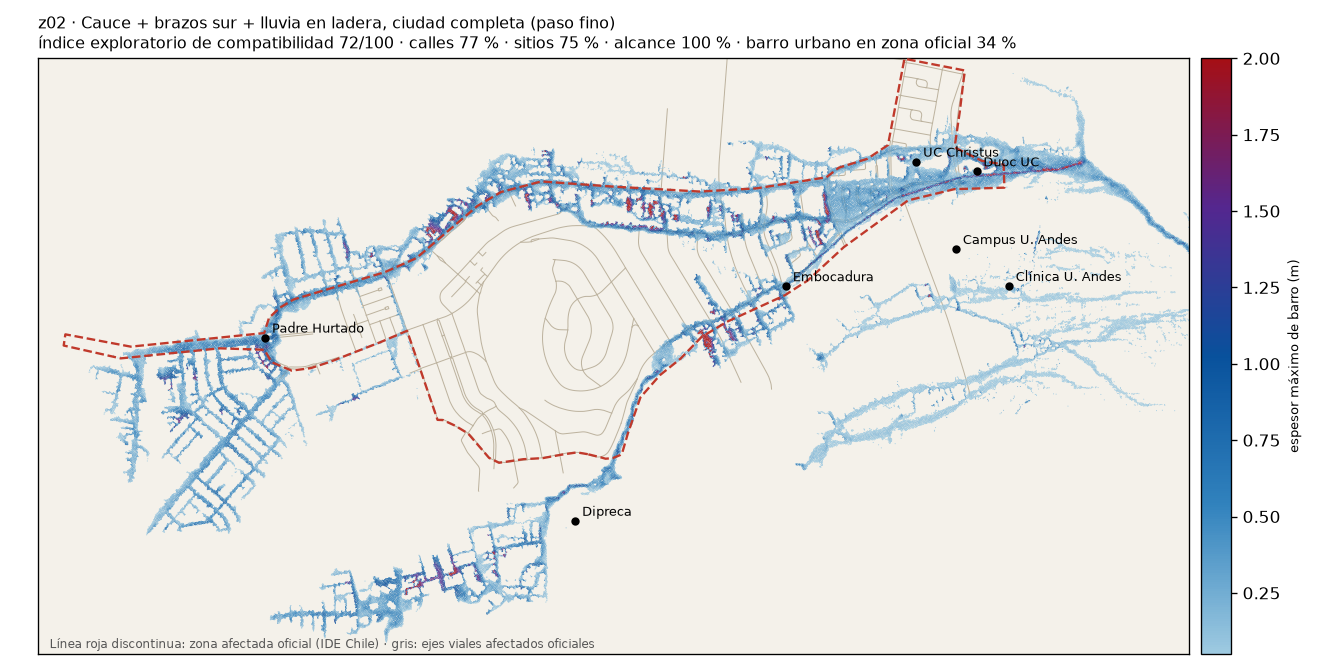
\includegraphics[width=\textwidth]{anexo/z02}\caption{Simulación z02 (cauce principal, brazos sur y lluvia en la ladera, paso de tiempo fino) sobre la zona afectada oficial de IDE Chile (línea roja discontinua) y los ejes viales afectados (gris) \citep{bbnn2026visor}. Colores: espesor máximo simulado.}\label{fig:ide}\end{figure}

\subsection{Ronda del 11 de octubre y prueba con observaciones reservadas}\label{sec:res-ronda}
\paragraph{Ensayos sobre la extensión y el doble conteo.} Cada ensayo cambió un factor de la hipótesis principal:
\begin{itemize}
\item \textbf{Barro algo más concentrado} (v25, $C_v=0{,}43$): no reduce el barro fuera de la zona afectada oficial (fracción dentro de la zona: 0,346, frente a 0,344 en z02).
\item \textbf{Mayor rugosidad fuera de las calles} (v27; $K=800$ y $n=0{,}08$): es el único que la reduce algo (0,388).
\item \textbf{Lluvia aplicada solo fuera de las cuencas aportantes} (v28): elimina el doble conteo sin cambiar los indicadores. La afectación junto a la Clínica Universidad de los Andes se mantiene (\SI{0,15}{m}).
\item \textbf{Reología por zona} (v29; $C_v=0{,}27$ en el faldeo): no cambia los componentes del índice.
\end{itemize}
En los cuatro, el componente «sitios» llega a 1,00 porque el punto de control del campus supera \SI{5}{cm} con el paso de tiempo normal (\SIrange{0,06}{0,15}{m}); en las referencias con paso fino disponibles para esa selección, ese punto queda en \SI{0,01}{m} (v19, z02). La verificación posterior propia de v29 (z29) sí mantiene el punto mojado (sección~\ref{sec:res-posterior}). Según una regla registrada antes de elegir el candidato (protocolo de validación, enmienda~1), ese componente se calcula sin el punto del campus. Así, los índices de 78--79 quedan en 72--73. Todas las configuraciones empatan dentro de tres puntos, y se selecciona z02, verificada con paso fino.

\paragraph{Microsimulaciones del campus.} Se ensayaron desbordes de \SI{20}{m^3/s} y \SI{40}{m^3/s} en la parte alta de Álvaro del Portillo, con barros de $C_v$ 0,25 a 0,40 y triángulos de \SI{8}{m^2} (m20, mk20, ml20, ml40). En todos, el flujo baja por la avenida y sale del dominio sin alcanzar la Biblioteca. El punto de desborde queda fuera de la cuenca local de la Biblioteca, a unos \SI{220}{m} de su límite, de modo que con este relieve ese flujo drena hacia otro lado. Las variantes de escorrentía generada dentro de esa cuenca local y de un camino de entrada que el terreno de \SI{30}{m} no resuelve se ensayaron después: las microsimulaciones y m36 reproducen la entrada por el claro al patio (sección~\ref{sec:res-posterior}). Su validación independiente permanece sin probar (sección~\ref{sec:conclusiones}).

\paragraph{Prueba con observaciones reservadas.} El procedimiento fue:
\begin{itemize}
\item \textbf{Reserva y métrica previas.} Antes de cruzarla con el modelo, se reservaron los 49 equipamientos afectados de la capa oficial que no coinciden con recintos de ajuste. Se fijó la métrica: fracción de puntos con barro simulado de más de \SI{5}{cm} a \SI{15}{m} o menos. El criterio favorable era al menos 0,70 y superar a las referencias v01 (solo cauce principal) y e03 (solo desborde en la embocadura).
\item \textbf{Ejecución única.} La prueba se ejecutó una sola vez sobre el candidato congelado.
\item \textbf{Resultados.} z02 alcanza 19 de 49 puntos (0,39), v01 los mismos 19 y e03 ninguno.
\end{itemize}
\textbf{El resultado es desfavorable.} Se informa sin modificar el modelo. En un diagnóstico posterior, que no cambia el veredicto:
\begin{itemize}
\item la distancia mediana a la celda con barro más cercana es de \SI{32}{m};
\item 16 puntos quedan a más de \SI{100}{m};
\item z02 moja cerca del \SI{20}{\percent} del área de la zona afectada oficial y el \SI{32}{\percent} de sus predios afectados.
\end{itemize}
Es decir, además de extenderse fuera de la zona afectada oficial, la reconstrucción deja sin barro partes importantes de ella. Parte de los puntos no alcanzados corresponden a instalaciones de servicio; su inclusión en la capa oficial no permite inferir el proceso físico de afectación. La prueba es solo parcialmente independiente, porque los puntos están en la zona usada por el índice.

\subsection{Ensayos posteriores a la prueba reservada}\label{sec:res-posterior}
Los ensayos de esta sección terminaron después de congelar el candidato y ejecutar la prueba reservada (sección~\ref{sec:res-ronda}). Sus resultados son de ajuste y no modifican el veredicto de esa prueba. Cualquier nueva selección requerirá observaciones reservadas nuevas.

\paragraph{Casas porosas.} En v26 los edificios de la zona afectada oficial dejan entrar el barro y lo retienen: piso a la cota del terreno más \SI{0,3}{m}, con alta resistencia. Con esta representación:
\begin{itemize}
\item la fracción del barro urbano dentro de la zona afectada oficial sube de 0,34 a 0,54;
\item el modelo moja el \SI{36}{\percent} de la zona afectada oficial (\SI{20}{\percent} en z02) y el \SI{40}{\percent} de sus predios afectados;
\item se cumplen los cuatro criterios originales.
\end{itemize}
La repetición con paso fino (z26) confirma un IEC de 76/100, y con la mitad de la resistencia (v30) el resultado casi no cambia. Como contrapartida, al retener barro en los lotes, el espesor junto a la urgencia de la Clínica UC Christus baja a \SI{0,30}{m}, frente a cerca de \SI{1}{m} informado por Cadena 3.

\paragraph{Faldeo más líquido.} Con la reología por zona ($C_v=0{,}27$ en el faldeo), el punto de control del campus se moja también con paso fino (\SI{0,09}{m} en z29), a diferencia de z02 (\SI{0,01}{m}). El IEC verificado es 78/100.

\paragraph{Cuadratura de la concentración.} Se usaron cinco nodos de Gauss para $C_v=0{,}20+0{,}30X$, $X\sim\mathrm{Beta}(3,2)$, sobre la configuración sin doble conteo. Los valores, condicionados a esa distribución de creencia y sin ser probabilidades de inundación, son:
\begin{itemize}
\item área esperada con más de \SI{5}{cm}: \SI{169}{ha} (\SI{144,5}{ha} mojadas en todos los nodos y \SI{192,3}{ha} en alguno);
\item espesor máximo esperado promediado: \SI{0,38}{m}, con una desviación entre nodos de \SI{0,027}{m};
\item IEC entre 71 y 73 en todo el rango.
\end{itemize}
La concentración mueve sobre todo los bordes de la extensión, no los espesores.

\paragraph{Campus y Av.\ La Plaza Sur.} El autor aportó cinco tipos de información:
\begin{itemize}
\item un video publicado por Meganoticias a las 18:16 del 8 de octubre \citep{meganoticias2026uandes}, con agua turbia que baja del bosque y llena un patio hundido junto a un edificio del campus (espesor estimado visualmente en este estudio: unos \SIrange{15}{35}{cm} según las bancas);
\item la ubicación de ese patio y del claro por donde entra el agua;
\item imágenes de Street View que muestran La Plaza Sur con dos calzadas a distinto nivel (aproximadamente \SI{1,5}{m});
\item 81 puntos con cota de Google Earth (diferencia con el modelo: \SI[uncertainty-mode=separate,retain-explicit-plus=true]{+1,1 +- 1,8}{m});
\item los trazados de un camino de tierra recto que baja del cerro a La Plaza Sur y de una entrada secundaria a un estacionamiento.
\end{itemize}
Con microsimulaciones (triángulos de \SI{8}{m^2}, lluvia de \SI{35}{mm/h} durante una hora y agua turbia, $C_v=0{,}10$) se obtuvo lo siguiente:
\begin{itemize}
\item el desborde simulado de Álvaro del Portillo no llega al patio con ninguno de los fluidos ensayados: el punto de desborde queda fuera de su cuenca local;
\item la lluvia local sobre el terreno sin modificar deja \SI{0,15}{m} en el patio. Un lomo de \SI{0,3}{m} del relieve, menor que su precisión vertical, desvía el agua del claro a otro punto bajo;
\item al tallar el paso del claro al patio, el patio llega a \SIrange{0,17}{0,30}{m}, dentro del rango del video;
\item al tallar la calzada baja de La Plaza Sur, la avenida tiene más de \SI{5}{cm} en el \SIrange{81}{87}{\percent} de sus puntos, frente al \SIrange{12}{20}{\percent} sin tallar. Es compatible con lo que El Dínamo atribuye a Senapred sobre las calles más afectadas;
\item el camino del cerro agrega agua donde llega a la avenida.
\end{itemize}
La configuración resultante supone escorrentía turbia de la ladera y del cerro: caminos de tierra, un \emph{bike park} con pistas desnudas y la superficie clasificada como quemada. En el modelo, la avenida encauza el agua hacia el norte y esta entra a la universidad por el claro. Se representa con propiedades distintas del barro espeso de la rama principal; no se identifica así el proceso ocurrido durante el evento. Los tallados son representaciones gruesas basadas en observaciones aportadas, no mediciones.

\paragraph{Hipótesis integrada.} v32 reúne lo anterior a escala de ciudad:
\begin{itemize}
\item casas porosas;
\item faldeo con $C_v=0{,}10$ y resto con $C_v=0{,}40$;
\item camino, La Plaza Sur y entradas a la universidad tallados;
\item lluvia de \SI{35}{mm/h} sobre todo el faldeo, fuera de las cuencas aportantes.
\end{itemize}
Resultados de v32:
\begin{itemize}
\item IEC bruto de 82/100: calles 0,77; sitios 1,00; alcance 1,00; zona afectada oficial 0,51. Cumple los cuatro criterios originales;
\item el punto del campus llega a \SI{0,61}{m};
\item La Plaza Sur tiene más de \SI{5}{cm} en el \SI{46}{\percent} de sus puntos;
\item el agua llega por el claro al patio (\SI{0,07}{m}) y al estacionamiento (\SI{0,05}{m}). Es menos que en las microsimulaciones; la diferencia de resolución se examinó después con m36.
\end{itemize}
La repetición con paso fino (z32) mantiene el IEC en 82/100 y el campus en \SI{0,61}{m}: el resultado queda verificado. Está condicionado, además, a una lluvia de \SI{35}{mm/h} durante una hora, que supera la intensidad medida (máximo de aproximadamente \SI{22}{mm/h} en \SI{30}{min} en Río Molina).

\paragraph{Sensibilidad a la lluvia.} El CR2 informa registros de Río Molina de unos \SI{32}{mm} entre las 15:00 y las 19:00, con un máximo de \SI{10,9}{mm} en \SI{30}{min}. Con la lluvia medida (v33: \SI{8}{mm/h} durante \SI{4}{h}):
\begin{itemize}
\item el IEC de la hipótesis integrada baja a 79/100 y la fracción dentro de la zona afectada oficial a 0,41: la lluvia larga moja más superficie fina fuera de ella;
\item el campus sigue mojado (\SI{0,48}{m});
\item en La Plaza Sur y el patio la señal se debilita, aunque la malla de ciudad la subestima.
\end{itemize}
A escala de detalle, con \SIlist{15;25;35}{mm/h}, el mecanismo La Plaza Sur $\rightarrow$ claro $\rightarrow$ patio aparece en los tres casos: el patio queda en \SIrange{0,12}{0,17}{m} y La Plaza Sur se moja en el \SIrange{41}{87}{\percent}. No depende de excluir las cuencas aportantes ni del aporte de las quebradas cortas del sur. Por eso los resultados de ajuste se informan como rango según la lluvia: IEC de 79 a 82.

Un primer intento (v31), que inyectaba el cauce principal aguas arriba de una franja densa de árboles señalada por el autor, se descartó: el punto de inyección no estaba en el fondo de la quebrada y el flujo se escapó hacia el norte.

\paragraph{Lluvia con su distribución temporal registrada.} Con la lluvia de Río Molina cada \SI{30}{min} (\SI{31,8}{mm} entre las 15:00 y las 19:00, digitalizada de la figura del CR2 y consistente con sus totales), con el pico del hidrograma al final del tramo más intenso (p34b, corregida):
\begin{itemize}
\item la hipótesis integrada obtiene un IEC de 81 (calles 0,77; zona afectada oficial 0,48);
\item el campus llega a \SI{0,49}{m} y La Plaza Sur tiene barro en el \SI{33}{\percent} de sus puntos;
\item la superficie con más de \SI{5}{cm} es de \SI{222}{ha}.
\end{itemize}
El pulso concentra el agua y moja menos superficie fuera de la zona afectada oficial que la misma lluvia repartida en \SI{4}{h} (79).

Con triángulos de \SI{8}{m^2} en el campus y La Plaza Sur (m36), la simulación de ciudad reproduce el mecanismo de las microsimulaciones:
\begin{itemize}
\item el patio llega a \SI{0,17}{m}, dentro del rango del video, y el claro a \SI{0,19}{m};
\item La Plaza Sur tiene barro en el \SI{58}{\percent} de sus puntos;
\item el resto de la ciudad casi no cambia (IEC 82; \SI{220}{ha} mojadas).
\end{itemize}
La diferencia entre escalas se debía a la resolución de la malla, no al proceso. m36 se lanzó antes de la corrección del paso de tiempo y tiene un residuo de \SI[retain-explicit-plus=true]{+0,6}{\percent}.

\paragraph{Artefacto numérico detectado y corregido.} En las corridas de este grupo (p34, d39, f35, f38, arc y art), los hidrogramas comienzan a las \SI{2,8}{h} para coincidir con el pulso de lluvia. Mientras tanto, el dominio está casi seco y el modelo toma pasos de tiempo muy grandes sobre la película de lluvia. Entre los minutos 1 y 2, la corrección de profundidades negativas creó unos \SI{7500}{m^3} en el faldeo: un residuo de balance de \SI[retain-explicit-plus=true]{+2,1}{\percent} (\SI[retain-explicit-plus=true]{+3,1}{\percent} en las corridas sin incendio). Las seis corridas comparten el artefacto, de modo que las comparaciones entre ellas siguen siendo válidas. Con un paso de tiempo máximo de \SI{0,5}{s}, el residuo vuelve a cero. Las repeticiones corregidas (p34b, f35b y f38b) tienen un residuo de \SI{0,00}{\percent} y confirman las conclusiones: los valores cambian en pocas hectáreas y centésimas de metro. Se informan los valores corregidos.

\paragraph{Obstáculo hipotético de árboles.} El autor marcó una línea de árboles que baja por la quebrada principal (\SI{1046}{m} a \SI{994}{m} de cota en unos \SI{720}{m}) y una acumulación al final, poco antes de la salida al abanico. Se talló un cauce por esa línea, con el hidrograma del cauce principal inyectado aguas arriba (arc), y se agregó la acumulación como un obstáculo de altura supuesta de \SI{3}{m} (art). Resultados del modelo:
\begin{itemize}
\item el obstáculo supuesto no desvía el flujo simulado hacia el sur: Álvaro del Portillo y el campus tienen la misma superficie mojada en ambos casos (\SI{20,2}{ha});
\item retiene y reparte barro junto al abanico (unas \SI{59}{ha} más mojadas) y el barro llega menos lejos hacia el poniente (unas \SI{70}{ha} más secas);
\item el IEC casi no cambia (78 frente a 79).
\end{itemize}

\paragraph{\emph{Bike park}.} Con el dominio ampliado al este y al sur, con lluvia de \SI{25}{mm/h} y agua turbia, se comparó el terreno con y sin la pista principal del \emph{bike park} tallada hasta el inicio del camino del cerro (mrbt y mrbc). Los resultados son idénticos:
\begin{itemize}
\item La Plaza Sur con barro en el \SI{78}{\percent} de sus puntos;
\item \SI{0,26}{m} al final del camino, \SI{0,14}{m} en el claro y \SI{0,11}{m} en el patio.
\end{itemize}
En el modelo, con este relieve, el agua de la superficie del \emph{bike park} escurre hacia el camino, con o sin la pista tallada. Incluir toda la ladera alta en la lluvia sí agrega agua: frente a mrd25, La Plaza Sur pasa del \SI{69}{\percent} al \SI{78}{\percent}. El aporte de sedimento de las pistas no puede evaluarse, porque el modelo no simula erosión.

\paragraph{Porosidad por tamaño.} Si solo las casas de \SI{250}{m^2} o menos dejan entrar el barro (d39), el espesor junto a la Clínica UC Christus sigue en \SI{0,31}{m}. El menor espesor calculado allí se debe al almacenamiento representado en las casas de aguas arriba, no al tamaño de los edificios.

\subsection{Campus de la Universidad de los Andes}\label{sec:res-campus}
El vicerrector de la universidad ubicó el desborde en la quebrada del costado norte del campus, que colinda con General Blanche, por donde bajó la masa de barro \citep{cooperativa2026}, y Carabineros ubicó la zona cero en Álvaro del Portillo con Av.\ La Plaza \citep{latercera2026zonacero}; un video difundido en redes muestra barro en el Aula Magna \citep{quintaconectado2026}. En el modelo con el brazo sur por el cauce oficial (v19), el barro llega a la parte alta de Álvaro del Portillo (\SI{0,49}{m} donde termina el cauce y \SI{0,13}{m} en la avenida) y baja por ella hacia La Plaza y General Blanche, en concordancia con ambos relatos. No cruza, en cambio, el bosque que separa la avenida de la biblioteca, aunque el terreno desciende de \SI{936,5}{m} a \SI{927,4}{m} hacia una depresión junto al edificio. Se ensayaron inicialmente tres mecanismos: (i) \emph{aporte de quebradas secundarias}: la delimitación sobre el terreno asigna a la biblioteca una cuenca local de \SI{11,3}{ha}, ajena a las cuencas aportantes, de la que solo el \SI{57}{\percent} recibe lluvia en las simulaciones principales; (ii) \emph{escorrentía más líquida en el faldeo}: en las imágenes del campus citadas no se distinguen piedras ni escombros urbanos; se ensayó por ello un flujo más diluido que en la rama principal; y (iii) \emph{redistribución local} por taludes, senderos y accesos. Para ello se usaron microsimulaciones locales de unos \SI{800}{m} $\times$ \SI{720}{m} con triángulos de \SI{8}{m^2}, con desbordes de \SI{10}{m^3/s} a \SI{40}{m^3/s} en la parte alta de Álvaro del Portillo, barros de $C_v$ 0,25, 0,30 y 0,40, y lluvia sobre toda la cuenca local. También se usó una simulación de la ciudad completa (v29) con reología por zona: $C_v=0{,}27$ en el faldeo y $C_v=0{,}43$ en el resto, más la lluvia aplicada solo fuera de las cuencas aportantes. La reología por zona es una representación intermedia: asigna un barro distinto según la ubicación, pero no representa la evolución de la concentración durante el recorrido. Los ensayos posteriores reprodujeron la entrada por el claro al patio; m36 calcula \SI{0,17}{m} en el patio y moja el \SI{58}{\percent} de La Plaza Sur (sección~\ref{sec:res-posterior}).

\subsection{Terreno anterior}\label{sec:res-terreno}
El dominio cubre \SI{5,9}{km} por \SI{3,4}{km} con una retícula de \SI{4}{m}. Contiene 1.103 edificios representados como bloques, con altura media de \SI{6,2}{m} y máxima de \SI{39}{m}: 82 alturas obtenidas de la diferencia entre superficie y terreno, 26 de los pisos registrados y 995 supuestas en \SI{6}{m}. Se excluyeron cuatro polígonos que corresponden a recintos (complejos deportivos y un centro comercial) y no a volúmenes construidos. En el terreno base, el cauce abierto del parque lineal entre el abanico y Francisco Bulnes Correa queda prácticamente plano (relieve transversal de $\pm\SI{0,5}{m}$). En el terreno fotogramétrico del año 2014 \citep{hussain2021}, con resolución efectiva de \SI{8}{m} a \SI{10}{m}, el cauce aparece como una depresión de \SI{1}{m} a \SI{4,5}{m} respecto de sus márgenes. Ese terreno presenta un desfase vertical de \SI{26,7}{m} (diferencia entre referencias elipsoidal y geoidal) y depresiones espurias, que se corrigieron antes de usarlo.

\subsection{Verificación numérica}\label{sec:res-verif}
\paragraph{Equilibrio del depósito.} Al detenerse sobre un plano de pendiente 0,05, el depósito satisface el criterio de fluencia: el residuo local $r=\rho_m g h|\nabla(z+h)|/\tau_y$ tiene mediana y percentil 95 iguales a 1,00, sin celdas con $r>1{,}05$. El espesor teórico de reposo es $h_c=\SI{0,1200}{m}$ con $g=\SI{9,8}{m.s^{-2}}$.
\paragraph{Reinicio.} Al agregar mezcla aguas arriba, el frente avanza \SI{26}{m} más que en el control sin aporte. El control, sin embargo, también avanza \SI{19}{m} en \SI{900}{s}, y la deriva del frente detenido es de \SI{6,7}{m} en los últimos \SI{300}{s}. Ese deslizamiento residual proviene del paso fraccionado y disminuye al reducir el paso de tiempo.
\paragraph{Convergencia.} Con CFL~0,25, el alcance converge al refinar la malla: \SIlist{354;345,7;341,2}{m} para celdas de \SIlist{4;2;1}{m}, con un valor extrapolado de unos \SI{337}{m}. Con celdas de \SI{2}{m}, el alcance disminuye al reducir el número de Courant: \SIlist{431;374;346;328}{m} para CFL 1; 0,5; 0,25 y 0,1. Es una convergencia de primer orden, con un sesgo de \SI[retain-explicit-plus=true]{+30}{\percent} para CFL~1.
\paragraph{Convergencia en el dominio urbano.} En el terreno con las 42.018 huellas de edificios, la simulación de \SI{300000}{m^3} por el cauce principal se repitió con CFL~0,25. Respecto de CFL~1, la diferencia de espesor máximo tiene mediana de \SI{2}{mm} y percentil 95 de \SI{9}{mm}; el \SI{99}{\percent} de las celdas coincide en mojado o seco; la llegada del frente difiere en menos de \SI{20}{s}, y la distancia mínima a Padre Hurtado es la misma (\SI{96}{m}). En la simulación de ciudad, el frente se detiene por la geometría representada de calles y edificios y no por el deslizamiento residual del ensayo en plano. La comparación temporal urbana realizada no muestra un sesgo de esa magnitud en los indicadores examinados.
\paragraph{Doble conteo de la lluvia en la ladera.} La lluvia sobre la ladera se aplica en un polígono de \SI{1,048}{km^2} y aporta \SI{36680}{m^3} además de los hidrogramas. El \SI{74}{\percent} de ese polígono está fuera de las cuencas aportantes, cuya escorrentía ya entra por los hidrogramas; el \SI{26}{\percent} restante se superpone con parte de S1 (\SI{0,096}{km^2}) y con toda S2 (\SI{0,172}{km^2}), lo que cuenta dos veces unos \SI{9400}{m^3}, el \SI{2,8}{\percent} del volumen total, concentrados en el entorno de la Clínica Universidad de los Andes. La simulación v28 repite la hipótesis principal aplicando la lluvia solo fuera de las cuencas (\SI{27290}{m^3}) para cuantificar su efecto.
\paragraph{Balance de volumen.} En todas las simulaciones del dominio urbano, el volumen en la malla coincide con el aportado, menos el retirado por el colector y el que sale por los bordes, con un residuo menor a \SI{0,01}{\percent}. Hay excepciones documentadas. En las seis corridas con los hidrogramas desplazados (p34, d39, f35, f38, arc y art), la corrección de profundidades negativas creó entre un \SI{2,1}{\percent} y un \SI{3,1}{\percent} de masa (sección~\ref{sec:res-posterior}); se corrigió, y las repeticiones p34b, f35b y f38b dan \SI{0,00}{\percent}. En m36, con malla fina en el campus y lanzada antes de la corrección, el residuo es de \SI[retain-explicit-plus=true]{+0,6}{\percent}. En algunas microsimulaciones del campus con lluvia, el residuo llega hasta un \SI{3,2}{\percent}, y se informa en cada caso. Una versión anterior del borde de salida generaba masa espuria al llegar el frente al límite sur, con un aumento de hasta un \SI{20}{\percent}; esas simulaciones se descartaron y se repitieron con un borde de solo salida.

\subsection{Estimación independiente del volumen}\label{sec:res-volumen}
La delimitación sobre el modelo de elevación calcula una cuenca aportante de \SI{10,1}{km^2}: el cauce principal (\SI{8,04}{km^2}, relieve de \SI{1376}{m}), el cauce sur (\SI{1,90}{km^2}) y las quebradas menores (\SI{0,17}{km^2}). Con el balance lluvia--escorrentía, la mediana del volumen de mezcla es de \SI{151000}{m^3}, con percentiles 5 y 95 de \SI{67000}{m^3} y \SI{310000}{m^3}. En el cálculo inicial del modelo para cuencas quemadas \citep{gartner2014}, con severidad supuesta, la mediana fue de \SI{374000}{m^3}, con percentiles de \SI{61000}{m^3} y \SI{2,3e6}{m^3}; al usar la severidad estimada con dNBR se obtuvo \SI{148000}{m^3} (sección~\ref{sec:res-incendio}). Con \SI{151000}{m^3}, la relación de \citet{mizuyama1992} da $Q_p\approx\SI{230}{m^3/s}$.

Con el escenario de suelo saturado, la mediana sube a \SI{295000}{m^3}, con percentiles 5 y 95 de \SI{181000}{m^3} y \SI{468000}{m^3}. El límite superior calculado para la fusión de nieve es de unos \SI{15000}{m^3}, menos del \SI{5}{\percent}: el análisis satelital descrito no detectó manto previo en la parte despejada de la cuenca y la hipsometría calcula el \SI{90}{\percent} de su superficie bajo \SI{1800}{m}. En los escenarios de isoterma, cambia el área supuesta que recibe lluvia: si la cota de nieve se toma unos \SI{300}{m} bajo la isoterma, en el cálculo, una isoterma supuesta de \SI{2000}{m} deja \SI{8,2}{km^2} bajo lluvia (\SI{81}{\percent}), una de \SI{1800}{m}, \SI{6,0}{km^2} (\SI{59}{\percent}), y una de \SI{1500}{m}, \SI{1,7}{km^2} (\SI{16}{\percent}); con la isoterma informada para el 8 de octubre se supone lluvia sobre los \SI{10,1}{km^2}. Con la misma lluvia supuesta, los escenarios de isoterma típica calculan entre un \SI{20}{\percent} y un \SI{40}{\percent} menos de agua en el pulso.

\subsection{Severidad estimada del incendio y escenarios de volumen}\label{sec:res-incendio}
La severidad se calculó con el índice dNBR de Sentinel-2 \citep{keybenson2006}, comparando una escena sin nubes del 23 de diciembre de 2025, seis días antes del inicio del incendio, con otra del 6 de febrero de 2026 (figura~\ref{fig:dnbr}). La distribución espacial coincide con la que publicó el CR2 \citep{cr2_2026}. De los \SI{10,1}{km^2} de las cuencas aportantes:
\begin{itemize}
\item \SI{8,2}{km^2} (\SI{82}{\percent}) muestran señal de quema (dNBR de 0,10 o más);
\item la severidad es mayoritariamente baja (\SI{2,8}{km^2}) o moderada-baja (\SI{4,5}{km^2});
\item solo \SI{1,0}{km^2} (\SI{10}{\percent}) es de severidad moderada-alta o alta, casi todo en el cauce principal.
\end{itemize}
Los umbrales de clase se calibraron en bosques de Norteamérica y la imagen posterior tiene cinco semanas de rebrote, por lo que la severidad puede estar subestimada en el matorral esclerófilo.

\emph{Corrección del volumen empírico.} El modelo de \citet{gartner2014} se había aplicado con una fracción de severidad moderada-alta supuesta entre \SI{30}{\percent} y \SI{90}{\percent} (sección~\ref{sec:res-volumen}). Con la severidad estimada por satélite para la entrada $B_{mh}$, su mediana de volumen de mezcla baja de \SI{374000}{m^3} a \SI{148000}{m^3}, con percentiles 5 y 95 de \SI{25000}{m^3} y \SI{858000}{m^3}. El balance lluvia--escorrentía no depende de ese supuesto.

\emph{Comparación de escenarios con y sin incendio.} En el balance de suelo saturado, el coeficiente de escorrentía se asignó por clase de severidad:
\begin{itemize}
\item $C_u$ entre 0,40 y 0,60 en lo no quemado;
\item $C_u$ más 0,05--0,15 en severidad baja, 0,15--0,30 en moderada-baja y 0,25--0,45 en moderada-alta o alta, por la hidrofobicidad y la pérdida de cobertura \citep{moody2013};
\item $C_v$ entre 0,30 y 0,50 con incendio y entre 0,20 y 0,35 sin incendio.
\end{itemize}
En el escenario sin incendio se asigna $C_u$ a toda la superficie de la cuenca. Estos incrementos son supuestos, no mediciones. Con ellos, el coeficiente efectivo pasa de 0,50 sin incendio a 0,66 con incendio, y el escenario sin incendio calcula para el pulso:
\begin{itemize}
\item el \SI{76}{\percent} del agua (\SIrange{70}{81}{\percent});
\item el \SI{62}{\percent} del volumen de barro (\SIrange{51}{76}{\percent}), es decir, una mediana de \SI{163000}{m^3} en vez de \SI{262000}{m^3};
\item el \SI{43}{\percent} de los sólidos (\SIrange{25}{74}{\percent}).
\end{itemize}
Con el modelo M1 de \citet{staley2017}, que estima la probabilidad de que una tormenta genere un flujo de detritos en una cuenca quemada, la lluvia de \SI{15}{min} inferida de Río Molina da una probabilidad mediana de 0,28 con incendio y de 0,07 sin él. Ese modelo fue calibrado en el oeste de Estados Unidos y su uso aquí es ilustrativo.

\emph{Respuesta del modelo de ciudad.} Se repitió la hipótesis integrada con la lluvia medida y el volumen sin incendio, es decir, los \SI{300000}{m^3} del modelo multiplicados por la razón mediana del balance sin y con incendio (0,62): \SI{187000}{m^3}, con $Q_p=\SI{172}{m^3/s}$ según la relación de \citet{mizuyama1992} (f35b, repetición corregida de f35), y además con un barro más fluido, $C_v=0{,}25$ (f38b, repetición corregida de f38). Frente a la misma configuración con incendio (p34b, corregida):
\begin{itemize}
\item la superficie con más de \SI{5}{cm} baja de \SI{222}{ha} a \SIrange{179}{193}{ha} (\SIrange{13}{19}{\percent} menos);
\item la fracción de calles con barro baja de 0,77 a 0,70--0,73;
\item el espesor junto a la Clínica UC Christus baja de \SI{0,30}{m} a \SIrange{0,19}{0,23}{m}.
\end{itemize}
El IEC queda en 80--82, frente a 81 con incendio. La métrica de la zona afectada oficial mejora cuando hay menos barro y compensa la pérdida de calles. Estos valores corresponden a las repeticiones corregidas (p34b, f35b y f38b).

\begin{figure}[htbp]\centering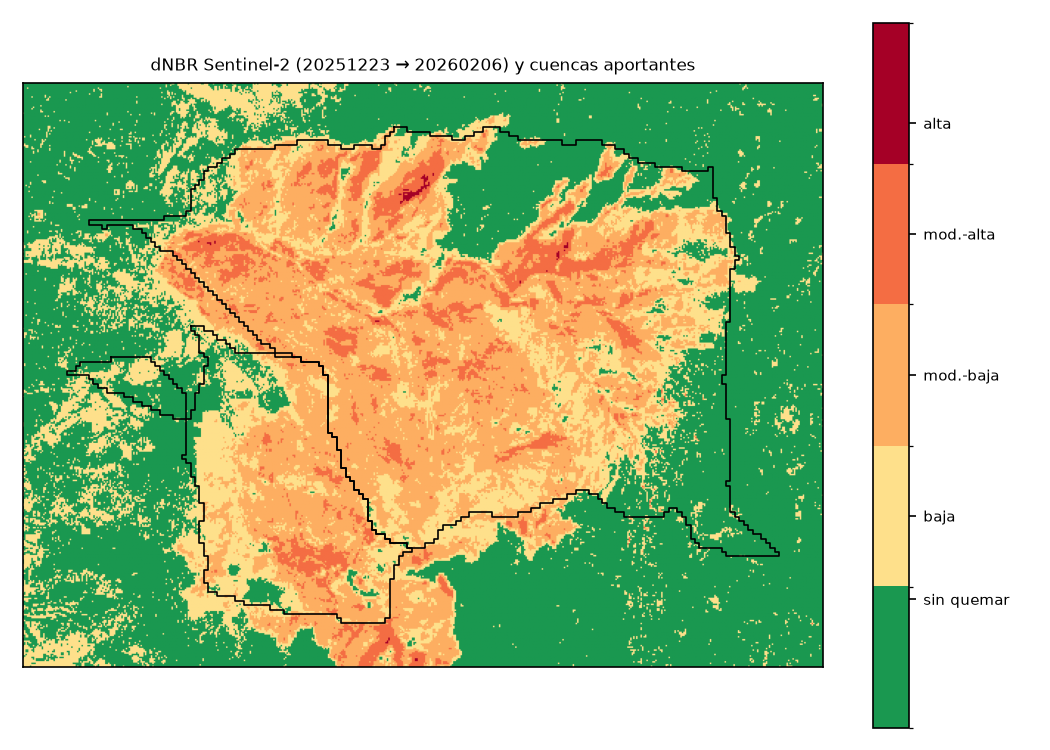
\includegraphics[width=.85\textwidth]{dnbr}\caption{Severidad estimada del incendio de diciembre de 2025 según el índice normalizado de área quemada diferencial (dNBR) de Sentinel-2 (23 de diciembre de 2025 y 6 de febrero de 2026) y límites de las cuencas aportantes (cauce principal al norte, brazo sur y quebradas menores).}\label{fig:dnbr}\end{figure}

\subsection{Cribado inicial con el terreno anterior}\label{sec:res-calib}
\begin{table}[htbp]\centering\small
\caption{Primera generación (9 de octubre de 2026), con el terreno anterior de 1.103 edificios: fracción de puntos de control con espesor máximo simulado mayor a \SI{5}{cm}, por calle, y espesor máximo en un radio de \SI{40}{m} de cada sitio. Las capacidades del colector son supuestas; no describen la obra real. Todas las simulaciones usan Glenwood~2b, $C_v=0{,}40$ y $Q_p=\SI{250}{m^3/s}$, salvo d03 ($Q_p=\SI{100}{m^3/s}$). LP: La Plaza (Álvaro del Portillo--Camino El Alba); GB: General Blanche (San Carlos de Apoquindo--Las Condesas); CEA: Camino El Alba; QH: Quebrada Honda; LPS: La Plaza Sur; UCC: Clínica UC Christus; CUA: Clínica Universidad de los Andes; Duoc: sede Duoc UC; dPH: distancia mínima del barro al cruce de General Blanche con Padre Hurtado.}\label{tab:hipotesis}
{\setlength{\tabcolsep}{4pt}\begin{adjustbox}{max width=\textwidth}\begin{tabular}{llrrrrrrrrr}\toprule
Hipótesis & $V$ (mil \si{m^3}) & LP & GB & CEA & QH & LPS & UCC (\si{m}) & CUA (\si{m}) & Duoc (\si{m}) & dPH (\si{m})\\\midrule
H3 & 80 & 0,87 & 0,86 & 0,61 & 0,00 & 0,00 & 0,22 & 0,00 & 0,42 & 1160\\
H1 & 150 & 0,91 & 0,92 & 0,85 & 0,00 & 0,00 & 0,42 & 0,00 & 0,55 & 366\\
H3 & 150 & 0,88 & 0,92 & 0,78 & 0,00 & 0,00 & 0,39 & 0,00 & 0,53 & 516\\
H3 & 300 & 0,91 & 0,93 & 0,96 & 0,00 & 0,00 & 0,42 & 0,00 & 0,54 & 4\\
H2 & 150 & 0,00 & 0,00 & 0,00 & 0,69 & 0,00 & 0,00 & 0,00 & 0,00 & 856\\
H4, $f_\mathrm{sup}=0{,}5$ & 150 & 0,88 & 0,88 & 0,57 & 0,66 & 0,00 & 0,26 & 0,00 & 0,46 & 1007\\
H4, $f_\mathrm{sup}=0{,}9$ & 150 & 0,88 & 0,91 & 0,68 & 0,54 & 0,00 & 0,35 & 0,00 & 0,52 & 816\\
H5 (H4 + lluvia de \SI{20}{mm/h}) & 150 & 0,88 & 0,88 & 0,57 & 0,66 & 0,00 & 0,26 & 0,06 & 0,46 & 1005\\
H1, cauce tallado, sin colector & 150 & 0,89 & 0,94 & 0,87 & 0,55 & 0,00 & 0,31 & 0,00 & 1,63 & 338\\
\quad ídem, colector \SI{10}{m^3/s} & 150 & 0,89 & 0,94 & 0,87 & 0,43 & 0,00 & 0,31 & 0,00 & 1,63 & 338\\
\quad ídem, colector \SI{30}{m^3/s} & 150 & 0,89 & 0,94 & 0,87 & 0,01 & 0,00 & 0,31 & 0,00 & 1,63 & 338\\
\bottomrule\end{tabular}\end{adjustbox}}
\end{table}

La tabla~\ref{tab:hipotesis} resume las simulaciones de cribado. Se observan cuatro regularidades:
\begin{enumerate}
\item \textbf{Corredores del abanico.} La Plaza, Mons.\ Álvaro del Portillo, Av.\ San Carlos de Apoquindo, el tramo alto de General Blanche y Camino El Alba superan el umbral en el \SIrange{85}{100}{\percent} de sus puntos en todas las hipótesis con salida en el abanico, para volúmenes entre \SI{80000}{m^3} y \SI{300000}{m^3}. Duoc UC y la Clínica UC Christus quedan alcanzados en todas ellas, con espesores de \SI{0,4}{m} a \SI{1,6}{m} y de \SI{0,2}{m} a \SI{0,4}{m}, respectivamente.
\item \textbf{Quebrada Honda.} En el cribado, esta calle solo supera el umbral cuando el flujo simulado sale a la superficie en la embocadura del colector de Francisco Bulnes Correa. Eso ocurre si se impone una fuente allí (H2, H4) o si el terreno representa el cauce abierto que conduce el flujo hasta la embocadura y el sumidero del modelo no lo retira. En esos ensayos basta con que salga allí el \SI{8}{\percent} del volumen.
\item \textbf{Capacidad del colector (terreno anterior; superado).} Con el cauce representado y solo 1.103 edificios, a la embocadura llegan \SI{12800}{m^3}, con un caudal máximo de \SI{16,5}{m^3/s}; en ese escenario, el sumidero del modelo con capacidad supuesta de \SI{30}{m^3/s} o \SI{100}{m^3/s} los retira y Quebrada Honda queda seca (\SI{1}{\percent}). Con la ciudad completa esta conclusión cambia: el caudal calculado sube a unos \SI{65}{m^3/s} y una capacidad supuesta de \SI{30}{m^3/s} deja flujo superficial (sección~\ref{sec:res-colector}). Con capacidad supuesta de \SI{10}{m^3/s}, el modelo calcula un desborde de unos \SI{2600}{m^3} y Quebrada Honda se moja en el \SI{43}{\percent} de sus puntos (figura~\ref{fig:colector}).
\item \textbf{Sector sur.} Ninguna de las simulaciones de la tabla~\ref{tab:hipotesis} moja la Av.\ La Plaza Sur ni el campus de la Universidad de los Andes. Solo la lluvia sobre la ladera oriente (H5) alcanza la Clínica Universidad de los Andes, con \SI{6}{cm} en su entorno, lo que coincide con la declaración de la clínica recogida por Radio La Señal de que la afectación fue exterior.
\end{enumerate}
Con el terreno anterior, ninguna simulación cumple los cuatro criterios de aceptación fijados de antemano (sección~\ref{sec:calib}). El criterio de sitios no se cumple en ninguna, porque no se alcanza el campus, y el de alcance no se cumple en las de \SI{150000}{m^3}.

\begin{figure}[htbp]\centering
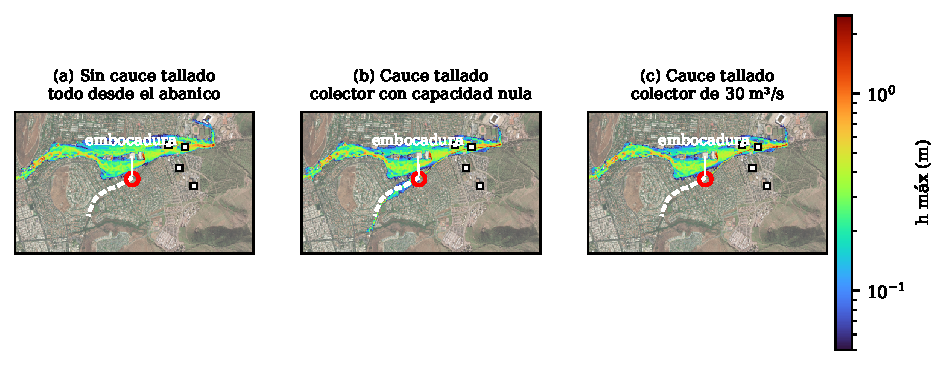
\includegraphics[width=\textwidth]{colector}
\caption{Primera generación (terreno anterior, 1.103 edificios; superada por la sección~\ref{sec:res-colector}). Espesor máximo simulado con \SI{150000}{m^3} saliendo en el abanico. (a) Terreno base: el flujo no alcanza Quebrada Honda (línea blanca discontinua). (b) Cauce del parque lineal tallado y sumidero del modelo con capacidad nula supuesta: el flujo que llega por el cauce a la embocadura (círculo rojo) desborda hacia Quebrada Honda. (c) Mismo terreno con capacidad supuesta del sumidero de \SI{30}{m^3/s}: el modelo retira el flujo que llega y Quebrada Honda queda seca. Los cuadrados indican los sitios con afectación informada por las fuentes de la sección~\ref{sec:evidencia}.}\label{fig:colector}
\end{figure}

\subsection{Contraste con información posterior a las hipótesis}\label{sec:res-contraste}
Después de formular las hipótesis se conocieron tres fuentes que permiten un contraste parcial, aunque no independiente de la prensa:
\begin{itemize}
\item \textbf{Versión preliminar recogida por El Desconcierto} \citep{eldesconcierto2026}: el medio recoge una versión del delegado presidencial sobre la obstrucción del ingreso a dos ductos paralelos en General Blanche y describe una interrupción del funcionamiento de la cámara de decantación de Francisco Bulnes Correa; también recoge un desborde del canal en esa calle informado por Carabineros. Son versiones de la fuente. En los escenarios ensayados, representar aportes superficiales en ambos sectores permite reproducir flujo en el abanico y Quebrada Honda, sin confirmar esas versiones ni el estado de las obras.
\item \textbf{Reporte técnico de Sernageomin sobre el aluvión del 31 de enero de 2026} \citep{sernageomin2026reterm}: describe un corredor único desde el Parque San Carlos de Apoquindo, por el sector de la Universidad de los Andes, hasta Quebrada Honda con Francisco Bulnes Correa, con continuación hacia la quebrada Apoquindo, el Hospital Dipreca y Paul Harris. El reporte describe el canal paralelo a Quebrada Honda colmatado de barro tras ese evento. Coincide con el recorrido del cauce que el modelo necesita representar. El dominio ampliado de la versión vigente ya incluye la continuación hacia Dipreca y Paul Harris.
\item \textbf{Mapa de prensa} \citep{chilevision2026mapa}: traza como vías del aluvión los ejes de Camino El Alba, General Blanche y Quebrada Honda hasta Padre Hurtado. Sobre esas líneas completas, la simulación considerada en ese contraste moja el \SI{92}{\percent} de Camino El Alba, el \SI{40}{\percent} de General Blanche y el \SI{27}{\percent} de Quebrada Honda. El tramo bajo de General Blanche, entre Las Condesas y Padre Hurtado, no se reproduce: el flujo simulado prefiere Camino El Alba en ese tramo.
\end{itemize}

Entre el 9 y el 10 de octubre se conocieron más datos, que se contrastaron sin modificar las simulaciones:
\begin{itemize}
\item \textbf{Lugares con ingreso de barro o agua.} Según las fuentes citadas, Senapred incluye la Av.\ La Plaza Sur entre las tres calles más afectadas; el campus de la Universidad de los Andes tuvo barro y personas retenidas, y la Clínica Universidad de los Andes, un ingreso menor de agua \citep{interferencia2026,cooperativa2026}. En el terreno con edificios, la simulación por el cauce principal no moja ninguno de esos tres puntos. La que agrega los brazos sur y lluvia sobre la ladera da \SI{0,14}{m} junto a la Clínica Universidad de los Andes y moja parte de La Plaza Sur, pero deja el campus con \SI{1}{cm}. Ambas reproducen la Clínica UC Christus (\SI{1,13}{m} a \SI{1,16}{m}, frente a cerca de \SI{1}{m} informado) y la sede Duoc UC (\SI{1,9}{m}).
\item \textbf{Evento del 31 de enero.} Según T13, con \SI{75}{mm} en \SI{1}{h} \SI{20}{min}, una intensidad mucho mayor que la del 8 de octubre, afectó \SI{8}{ha}, cerca de \SI{4}{km} de calles y 11 viviendas \citep{t13_2026mallas}, y el colector de Francisco Bulnes Correa «funcionó muy bien» según la alcaldesa \citep{latercera2026enero}. La diferencia entre los balances informados motiva los escenarios de saturación antecedente y material disponible; no permite establecer su contribución al evento ni compararla causalmente con la intensidad pico.
\item \textbf{Superficie afectada.} Las \SI{253}{ha} informadas por Chicureo Hoy \citep{chicureohoy2026} coinciden con el área del perímetro municipal publicado por la prensa (área calculada: \SI{253,0}{ha}). Es un perímetro de seguridad y no un mapa del barro: dentro de él el barro simulado ocupa cerca de \SI{40}{ha}, porque se concentra en las calles. No se usa para discriminar hipótesis.
\item \textbf{Hospital de la FACh.} Según Interferencia, se informó agua en su servicio de urgencias. Ninguna simulación llega a ese punto, unos \SI{1,3}{km} al norte del recorrido; no se usa como criterio de ajuste. El drenaje urbano por lluvia queda fuera del modelo y no se infiere aquí el origen de esa afectación.
\end{itemize}

\subsection{Indicadores en sitios críticos}\label{sec:res-indicadores}
Primera generación (terreno anterior, simulación e04; no comparable directamente con las simulaciones con la ciudad completa). En la simulación con el cauce tallado y el colector con capacidad nula supuesta, los máximos en un radio de \SI{40}{m} son los siguientes:
\begin{itemize}
\item Duoc UC: \SI{1,6}{m} de espesor, \SI{6,3}{m/s} y \SI{33}{kPa} de presión dinámica; el frente llega al minuto~4.
\item Cruce de General Blanche con San Carlos de Apoquindo: \SI{1,4}{m}, \SI{6,7}{m/s} y \SI{37}{kPa}, al minuto~7.
\item Clínica UC Christus: \SI{0,3}{m} y \SI{1,6}{m/s}, al minuto~9.
\item Embocadura de Francisco Bulnes Correa: \SI{1,6}{m} y \SI{3,9}{m/s}, al minuto~13.
\end{itemize}
Los minutos se cuentan desde el inicio del pulso. Con ese escenario, 170 edificios quedan con barro sobre \SI{5}{cm} junto a su fachada, 46 sobre \SI{0,5}{m} y 11 sobre \SI{1}{m}; 8 reciben una presión dinámica mayor a \SI{10}{kPa}. Estos valores tienen el sesgo de cribado ya señalado y no se han contrastado con mediciones.
